\documentclass[10pt]{report}
\usepackage{lingmacros}
\usepackage[normalem]{ulem}
%  Title Formatting 
\usepackage{titlesec}
% Removes paragraph indenting
\usepackage{parskip} 

% Figure labeling
\usepackage{hyperref}

\usepackage{amsmath}

% Font
\usepackage{tgpagella}

% Inline code
\usepackage{listings, lstautogobble}

\usepackage[labelfont=bf, labelsep=period]{caption}
\usepackage{graphicx}
\graphicspath{ {./images/} }

% Makes citations superscript
\usepackage[superscript,biblabel]{cite}
\usepackage{url}
\urlstyle{same}

\titleformat{\chapter}[block]
{\normalfont\huge\bfseries}{\thechapter.}{1em}{\Huge}
\titlespacing*{\chapter}{0pt}{-19pt}{0pt}

\lstset{language=Java,
	showstringspaces=false,
	breaklines=true,
	frameround=ffff,
	frame=single,
	autogobble=true
}

\begin{document}
	\begin{titlepage}
		\begin{center}
			\Large
			\textbf{A Survey of Procedural Generation Using Noise}
			
			\vspace{1.5cm}
			\normalsize
			\textbf{Michael Li}
			
			\vfill
			
			\textbf{DRAFT 2.2.0}
			
			\uline{Dianne Hansford, Ph.D \hfill Director}
			\vspace{1cm}
			
			\uline{Yoshihiro Kobayashi, Ph.D \hfill Second Committee Member}
			
			\vspace{3cm}
			
			
\includegraphics[scale=.5]{asu_barretthonors_horiz_rgb_maroongold_600ppi}
			
			\vspace{1.5cm}
			Ira A. Fulton Schools of Engineering
			
			School of Computing, Informatics, and Decision Systems Engineering
			
			Spring 2021
			
		\end{center}
	\end{titlepage}
	
	\chapter*{Abstract}
	
	\addcontentsline{toc}{chapter}{Abstract}
	Procedural content generation is a method of creating data algorithmically, often using stochastic models. These methods can be used to generate complex environments as opposed to manually creating environments by hand or by using photogrammetric techniques. Procedural generation can use a variety of techniques to achieve a stochastic or partially stochastic goal, including methods such as fractals, noise and deep learning. This paper will briefly survey procedural content generation techniques, how they work and their origins and history.
	
	\clearpage
	
	\tableofcontents
	
	\clearpage
	
	\let\clearpage\relax
	\chapter{Introduction}
	
		This paper surveys various methods of procedural generation of content and their applications in generating geological formations. While content can vary from terrain to creatures and stories in virtual worlds, the focus of this paper is primarily on terrain and more specifically geological formations. One of the most famous cases of this procedural generation for geological formations is Minecraft, which implements a modified version of Perlin noise in order to generate all of its worlds \cite{minecraft-gen}. Other examples include games such as The Elder Scrolls II: Daggerfall, which employs various forms of procedural generation to determine the location of non-player characters, the layout of dungeons, as well as the terrain itself \cite{daggerfall}. In more complex cases, procedural generation is used to create fake histories, with the more well-known example of Dwarf Fortress \cite{df-dev}. However, procedural generation's applications are not only limited to games. In The Lord of the Rings, many of the scenes with large amounts of characters were created using procedural generation, ensuring individual animations of the slightly differentiated characters \cite{massive}. While procedural generation is often described as being stochastic, in reality it is not entirely so. The majority of the techniques in procedural generation include some level of user control, as well as a specific input to use as a starting point for the equation. This input can be manipulated through a variety of different methods, some of which include noise-based methods, fractal methods as well as cellular automata. These methods can be mixed and matched in any number of ways as well, often to fine-tune different outcomes, or add variety to different content.
		
		The main topic that this paper will cover is the creation of geological formations through procedural generation, surveying some of the possible methods of doing so. A geological formation, or just formation is a body of rock that possesses some degree of internal consistency or distinctive features \cite{2005}. This allows geological formations to be separate from the region it is placed in while still being a landmark for the region it is being placed in. While procedural generation is differentiable in small regions, as a whole it is homogeneous, necessitating features such as formations to distinguish different regions. 
		
		\section{Definitions}
		PGC (procedurally generated content) refers to the use of algorithms to generate features including stories, characters, animals but specifically focusing on geological formations and terrain for this paper. To qualify as PGC, the result of the algorithm must be reproducible and modifiable. The reproducible criteria for PGC can be fulfilled by the use of deterministically random number generators, whereas the modifiable criteria are fulfilled by the use of parameters to modify the algorithm. While noise is related to PGC, it has several notable differences. Noise refers to the process often used for the creation of PGC, as it stochastically creates values. While these values can be reproducible similarly to PGC, noise focuses on the stochastic portion, while PGC often necessitates additional processing to generate the content portion. Fully randomized noise is not modifiable by the user and does not show any consistency in the end product. This can be seen below, in \autoref{fig:perlinnoise}, where the result of noise, can fulfill the requirements of PGC, PGC will not always fulfill the requirements of noise, due to the additional processing. 
		
		\begin{minipage}{\textwidth}
			\centering
			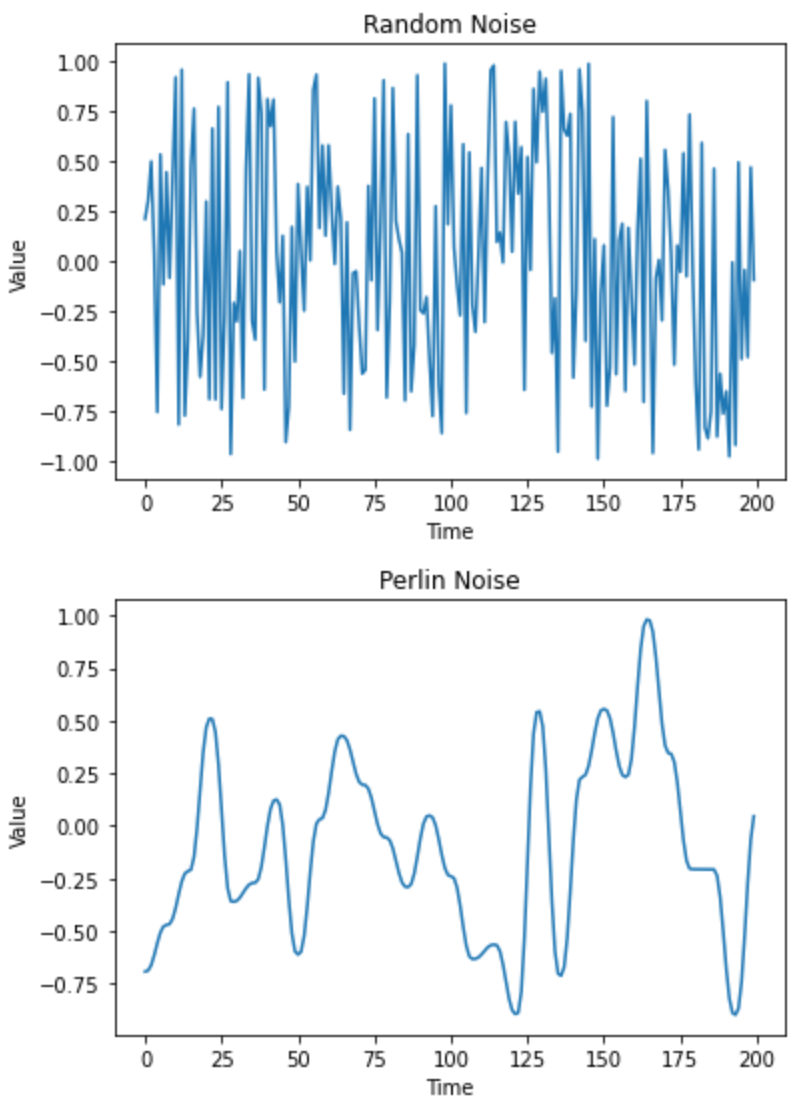
\includegraphics[scale=0.3]{perlinnoise}
			\captionof{figure}{Using the same set of input random numbers and the same algorithm, Perlin noise will always replicate this result.}
			\label{fig:perlinnoise}
		\end{minipage}

		
		\section{Random Number Generation and Seeding}
		
		PGC is often dependent on the use of random numbers, which has varying methods of generation in a computer. Random numbers may be generated through two methods through processes known as random bit generators, non-deterministically through the use of unpredictable physical processes, and computing numbers deterministically using an algorithm \cite{rng}. PGC algorithms follow the same methodology as the deterministically created random numbers. Similarly to deterministic random bit generators, in PGC a seed is a random number from which the rest of the algorithm will begin from. This seed number ensures the criteria for procedural generation to be reproducible, acting as a soft limit to the amount of randomness that can be created, since seeds are often relatively shorter in size, or constrained by the limits of memory. This seed number, as the starting point, will only have meaning in the context of the algorithm it is being used in - changing the algorithms manipulating the seed will change the entire output. This ensures regularity to the PGC, since any input number will result in the same set of outputs. By taking an input seed, it will be modified using an equation to obtain the output, possibly using additional random numbers created after the original seed. For PGC, an output can range from a character, to a story, to terrain, but this paper focuses on the generation of geological formations and the surrounding topography.
	
		\section{Methods Overview}
		This section will briefly cover some procedural generation techniques as well as an introduction to their methods and usage. These will be further elaborated on later, with additional details in their application and quirks in PGC. 
		
		Noise is a method of creating PGC, using the seeding method to manipulate and control the outcome. Lattice gradient noise is a commonly used and widespread form of noise. This form of noise creation works off of the premise of an integer lattice - a regularly spaced array of points in a square array\cite{integer-lattice}. One of the most well-known applications of this is Perlin noise, notably developed for use in Tron to create textures to allow for more realistic, interesting and believable effects and images \cite{ken-perlin}.Pseudo-random numbers are generated and evenly distributed across this lattice, then a low-pass filter is applied to smooth the edges between each of these points. A low-pass filter in this application helps to smooth the created lattice by averaging nearby values to reduce the difference between neighboring values, shown in \autoref{fig:lpf}. 
		
		\begin{minipage}{\textwidth}
			\centering
			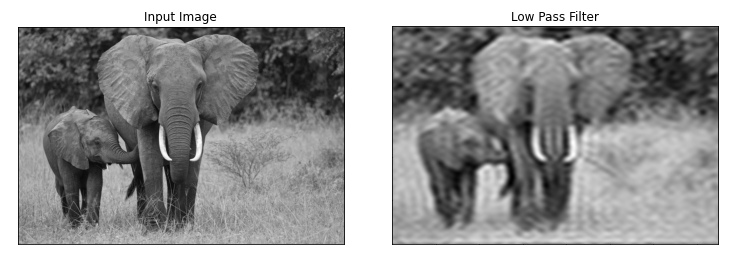
\includegraphics[scale=0.5]{lowpass}
			\captionof{figure}{Low-pass Filter Effect}
			\label{fig:lpf}
		\end{minipage}
		
		This creates a blurring effect, with fewer large value changes. The low-pass filter's effect is just creating the gradation between each of the lattice points. The result is an image such as the one shown in \autoref{fig:noise-ex}.
		
		\begin{minipage}{\textwidth}
			\centering
			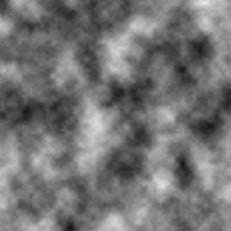
\includegraphics[scale=1]{lect14-perlin}
			\captionof{figure}{Perlin noise example. \cite{noise-ex}}
			\label{fig:noise-ex}
		\end{minipage}

		Using fractals is another approach at creating PGC. Fractal geometry being applied to landscapes began with studies of map data and research on the similarities between fractals and the data. Fractals prove as a relevant approach to representing geographical data due to the self-similarity and the subdivision of space, made easier by fractal surfaces \cite{doi:10.1111/j.1467-8306.1987.tb00158.x}. This provides a method of predicting the appearance and geometry of landscapes being studied. The technique works primarily from the subdivision of space combined with random numbers for each of the vertices created from the subdivision \cite{fractal-land}. In \autoref{fig:spatsub}, the four corner points act as the initially chosen vertices, and the vertices in the newly created plus shape are the vertices to randomly raise or lower. 
		
		\begin{minipage}{\textwidth}
			\centering
			
\includegraphics[scale=1]{landscapes}
			\captionof{figure}{Spatial Subdivision. \cite{fractal-land}}
			\label{fig:spatsub}
		\end{minipage}
		
		Similarly to Perlin noise, this technique often utilizes a seed random number to start from, to make the results reproducible. However, while fractals are very computationally efficient, the parameter that makes this seed is very sensitive to change. Very small changes will completely change the features of a map designed this way.
		
		\begin{minipage}{\textwidth}
			\centering
			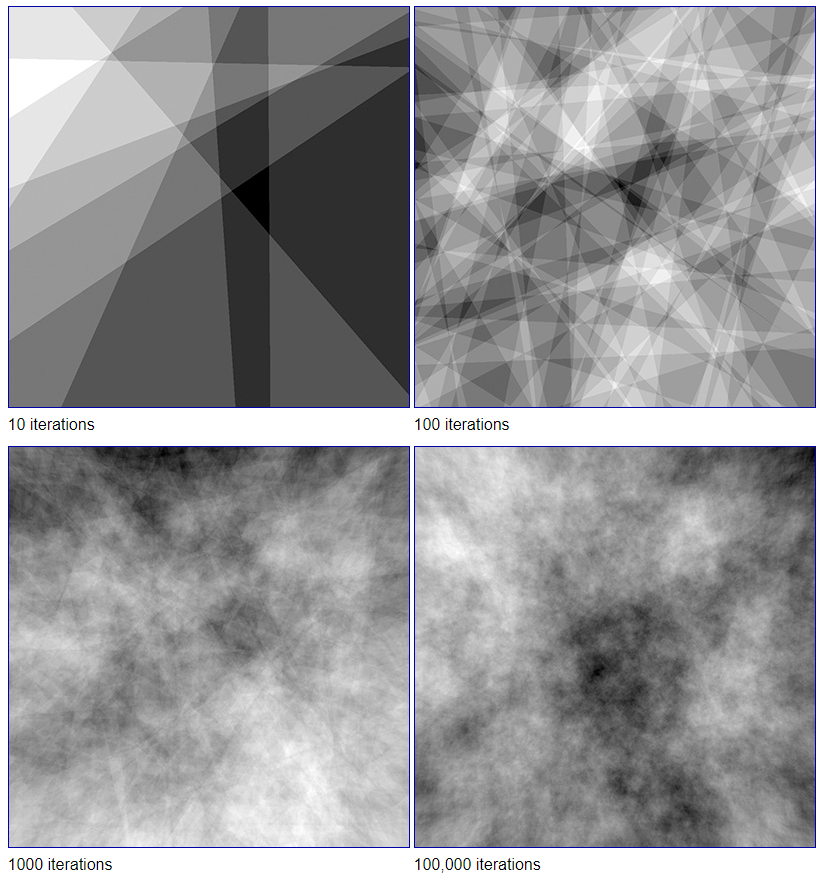
\includegraphics[scale=.5]{fractal-noise}
			\captionof{figure}{Fractal procedural generation example \cite{fractal-land}}
			\label{fig:fig2}
		\end{minipage}
		
		Another method of generating terrain revolves around the use of cellular automata. define cellular automata. Cellular automata works on a grid of cells, similarly to how noise is mapped, but instead of having a continuous value, the cells in this approach only have binary values, or similar. This approach relies on having the information of neighbors and the states of their neighbors to determine surrounding cells to then modify their states \cite{nature-of-code}. This can be used in conjunction with a tiling system to procedurally generate worlds, albeit with pre-determined cells for usage. This approach was demonstrated with a two-dimensional cave system to show the possibilities \cite{10.1145/1814256.1814266}.
		
		\section{Displaying Noise}
	
		Representing the data generated procedurally is another task with a variety of solutions. Some of these methods include pixel-based methods, polygons, and voxels. One common, simplistic way to represent the data generated is to use ASCII characters, or other types of two-dimensional data such as colored pixels to convey the scene that is being represented. In the case of Dwarf Fortress, the use of ASCII symbols is used to represent the elements within the game, shown in \autoref{fig:asciidf}.
		
		\begin{minipage}{\textwidth}
			\centering
			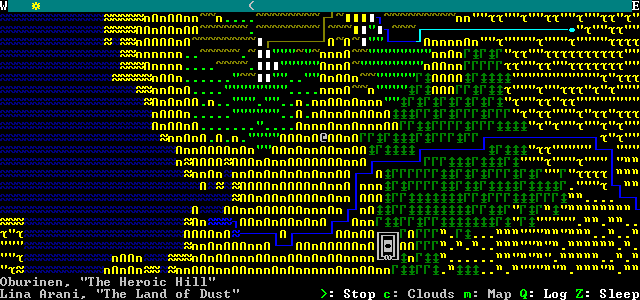
\includegraphics[scale=.5]{dwarf_fortress}
			\captionof{figure}{ASCII representation of PGC. \cite{df-dev}}
			\label{fig:asciidf}
		\end{minipage}
		
		Another one of the ways of representing three-dimensional objects is through the use of polygon meshes. These are created through polygons (typically triangles) joined by at least two vertices. These polygons are then represented by the coordinates of the vertices that compose them, while the space between the vertices acts as the viewable portion.
		
		In contrast to polygons representing faces of a geometry, voxels represent a value in space. This value represents a volume in space, and are placed in a regularly spaced grid of similar values. These valuesi n space can contain multiple data points, such as opacity, color, geometry (for example, cubes), among other things. Voxels are represented by their position relative to other voxels, allowing for easier representation of layers of geometry. An example of this voxel rendering can be found in the voxel space rendering engine, used for early flight simulator games. This used pre-generated height and color maps to determine which pixels would be visible on the screen, and at what height. The result is a fairly efficient method of rendering the player's perspective, at the cost of being unable to have more complex landscapes. In modern voxel based approaches, more complicated methods are used to render complex landscapes accurately.
		
		For areas of research and image-based approaches, a technique using kernels and convolutions may be applied. Kernels in this sense is a matrix that is convolved, or multiplied across another matrix in sections. Since these kernels sample a subset of a target matrix, it can be used to blur or sharpen features depending on the layout of the kernel. 
		
	\vspace{10pt}
	\let\clearpage\relax
	\chapter{Historical Usage}
		
		Perlin noise was developed for use in the movie industry, although it later became a foundation for many other procedural generation algorithms as it provided a lot of control as well as randomness to be used. It was developed in 1983 for use in the sci-fi movie Tron, to map textures onto computer generated surfaces for visual effects. Perlin noise has been used for many visual elements, ranging from the texture creation it was created for to particle effects such as fire, smoke and clouds, as well as landscapes and geological features. It has a variety of uses due to its ability to create a naturalistic appearance \cite{10.1145/325165.325247}.

		The beginning of the use of fractals to describe landscapes did not coincide with the conception of the term "fractal" by Mandelbrot in the 1970s, but developed in the decades to come as fractal geometry is able to capture surface topography in a way that other methods do not. While the potential of fractals to encapsulate and generate this geometry was noticed in the early 1990s, research at the time was still immature and unable to fully link the processes which create the forms captured by fractals. In terms of general landscapes, fractals were discovered to be able to imitate the self-similarity present in limited regions and limited ranges of scale in real landscapes. Some of the problems in furthering this research included the difficulty in researching and representing the dimensionality of natural terrain \cite{XU1993245}. However, this early PGC found its use in \emph{Star Trek II: The Wrath of Khan}to help develop planets that do not exist. This technology was used later on in an accompaniment to a SIGGRAPH paper to demonstrate more of the ability of fractals. This set the stage for later movies and projects such as \emph{The Last Starfighter} and \emph{Return of the Jedi} \cite{ibm-fractal}. 
		
		One of the earliest usages of PGC in video games was in Rogue \cite{rogue}. This initial attempt at generating a dungeon in a random manner addressed some of the differences between procedural generation and purely random generation, by introducing some level of control to the designer. Rogue addressed this by using a three by three grid to generate the layout of the level, with hallways randomly connecting the rooms. These rooms would have a variable size to increase the variety of levels producible by the algorithm. This technique in particular, was created to address the memory constraints of computers at the time, as even with this more mathematical and less memory intensive approach, levels would need to be cleared from memory when moving on to the next one \cite{rogue}.
		
	\vspace{10pt}
	\let\clearpage\relax
	\chapter{Height Maps}
	
		Perlin noise can be used to generate height maps to pseudo-randomly create geological formations. While height-maps have the advantage of being two-dimensional and less complicated to run, they have difficulty in rendering a variety of geological formations. Due to the two-dimensional nature of a height map, they are unable to render more complex features such as alcoves, arches, and any other three-dimensional feature. In terms of randomness, this can create a sort of uniformity in geometry, where the only features are hills and valleys. In signal terms, this means that noise is band-limited, where almost all of the energy of the noise is concentrated in a very small part of the frequency spectrum. An example of is shown in \autoref{fig:bandlimit}, where applying a band-limiting effect smooths out the function.
		
		\begin{minipage}{\textwidth}
			\centering
			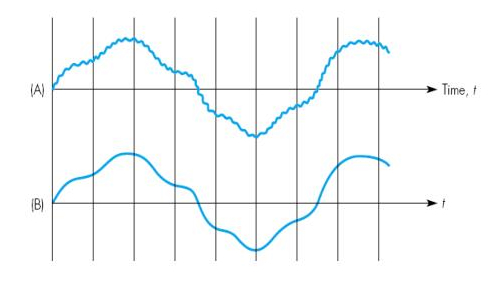
\includegraphics[scale=.5]{bandlimiting-filter}
			\captionof{figure}{Applying a band-limiting filter \cite{bandlimiter}}
			\label{fig:bandlimit}
		\end{minipage}
		
		The high and low frequencies of the original image would be blended out, and only the band-limited output image would remain, where the high and low frequencies contribute less to the total energy \cite{making-noise}. This can be mitigated to some extent by the use of layering differing octaves of noise to increase the amount of variation given by the noise. 
		
		The original implementation of Perlin noise was to create representations of various textures for objects, as well as representations of clouds, fire, water and stars among other things \cite{10.1145/325165.325247}. In other words, given an input point P, look at the surrounding points on the grid. In one dimension, this would be a series of line segments. 

		\begin{minipage}{\textwidth}
			\centering
			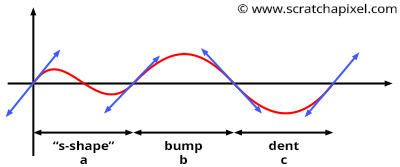
\includegraphics[scale=.5]{noise-value-vs-perlin3}
			\captionof{figure}{Perlin Noise gradients in one dimension \cite{pn-2}}
			\label{fig:pnoise1d}
		\end{minipage} 
		
		In two-dimensions there will be four points, due to the surrounding unit square, in three-dimensions there will be eight, due to the surrounding unit cube. Similarly to how in two dimensions space is parameterized by a lattice of integer squares, in three-dimensional space it is parameterized by a series of cubes. As Perlin noise scales up, this hypercube grows larger and larger in complexity, increasing the run time. For each of these surrounding grid points, Q, a pseudo-random gradient vector, G is chosen. This gradient is pseudo-random because, while the initial determination of the gradient vector's value is randomized, when inputting the same grid point the same gradient vector is chosen. In the calculation of Perlin noise, all of the points on the grid are located at zero. This attribute of Perlin noise can be seen in \autoref{fig:pnoise1d}. From there, the inner product is calculated between all of the surrounding grid points, the chosen point, and the gradient vectors. This results in G * (P - Q), giving 2\textsuperscript{n} values, where n represents the dimensionality of the grid. Then, interpolate between the values down to P, using an S-shaped cross-fade curve to weigh the interpolation in each dimension. This equation is shown below.
		
		\begin{lstlisting}[language=C]
			/* 3t^2 - 2t^3 */
			define s_curve(t) ( t * t * (3. - 2. * t) )
		\end{lstlisting}
		% cite? https://mrl.cs.nyu.edu/~perlin/doc/oscar.html#noise
		
		This was the original equation used for Perlin noise, but has since been superceeded. One of the problems with the previous equation used was that the second derivative of the function, \textbf{6-12t} is not zero at either \textbf{t=0} or \textbf{t=1}, causing discontinuities in the noise. Some of the effects of this are shown in \autoref{fig:pnartifact}. This led to the equation shown below to be used. 
		
		\begin{lstlisting}[language=Java]
			// 6t^5 - 15t^4 + 10t^3
			static double fade(double t) { return t * t * t * (t * (t * 6 - 15) + 10); }
		\end{lstlisting}
		% cite? https://mrl.cs.nyu.edu/~perlin/noise/
		
		This new equation led to an approximate ten percent speed increase compared to the original implementation. 
		
		\begin{minipage}{\textwidth}
			\centering
			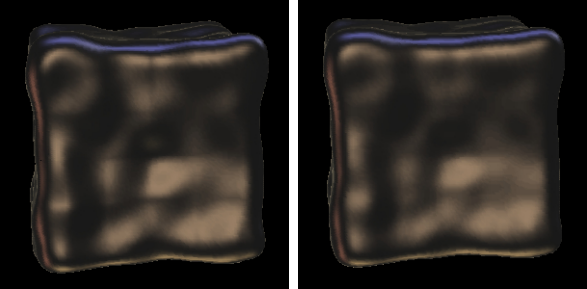
\includegraphics[scale=.5]{s-curve}
			\captionof{figure}{Removal of artifacting at t=0 and t=1 from revised interpolation function \cite{10.1145/566654.566636}}
			\label{fig:pnartifact}
		\end{minipage} 
		
		While Perlin noise saw great success, it was succeeded by algorithms such as Simplex noise, designed to alleviate some of the problems with Perlin noise. This included the computational complexity and the artifacting in the noise created. The artifacting in the noise appears from the necessity for the gradients to pass through zero, as shown in \autoref{fig:pnartifact}. This causes unavoidable artifacting in the noise. In addition, while Perlin noise's computational complexity is acceptable when in three-dimensional space and lower, it suffers greatly from increasing the dimensionality further.
	
	\vspace{10pt}
	\let\clearpage\relax
	\chapter{Image Based Methods}
	
		Some of the other uses of height maps include the voxel space rendering system, using voxel raster graphics to display three-dimensional geometry with low memory and processing requirements. This was developed in the early 90's, involving a height and color map to position the pixels on the screen. While this technique was not historically used with noise generating algorithms, the rendering system fits the requirements for the use of techniques such as two-dimensional Perlin noise. By using Perlin noise, the height and color maps can be generated at run-time instead of being created beforehand. An example of this is shown in \autoref{fig:pnvs}. At the time, displaying complex height-maps in three-dimensions was difficult computationally, and the voxel space technique allowed this to happen. 
		
		\begin{minipage}{\textwidth}
			\centering
			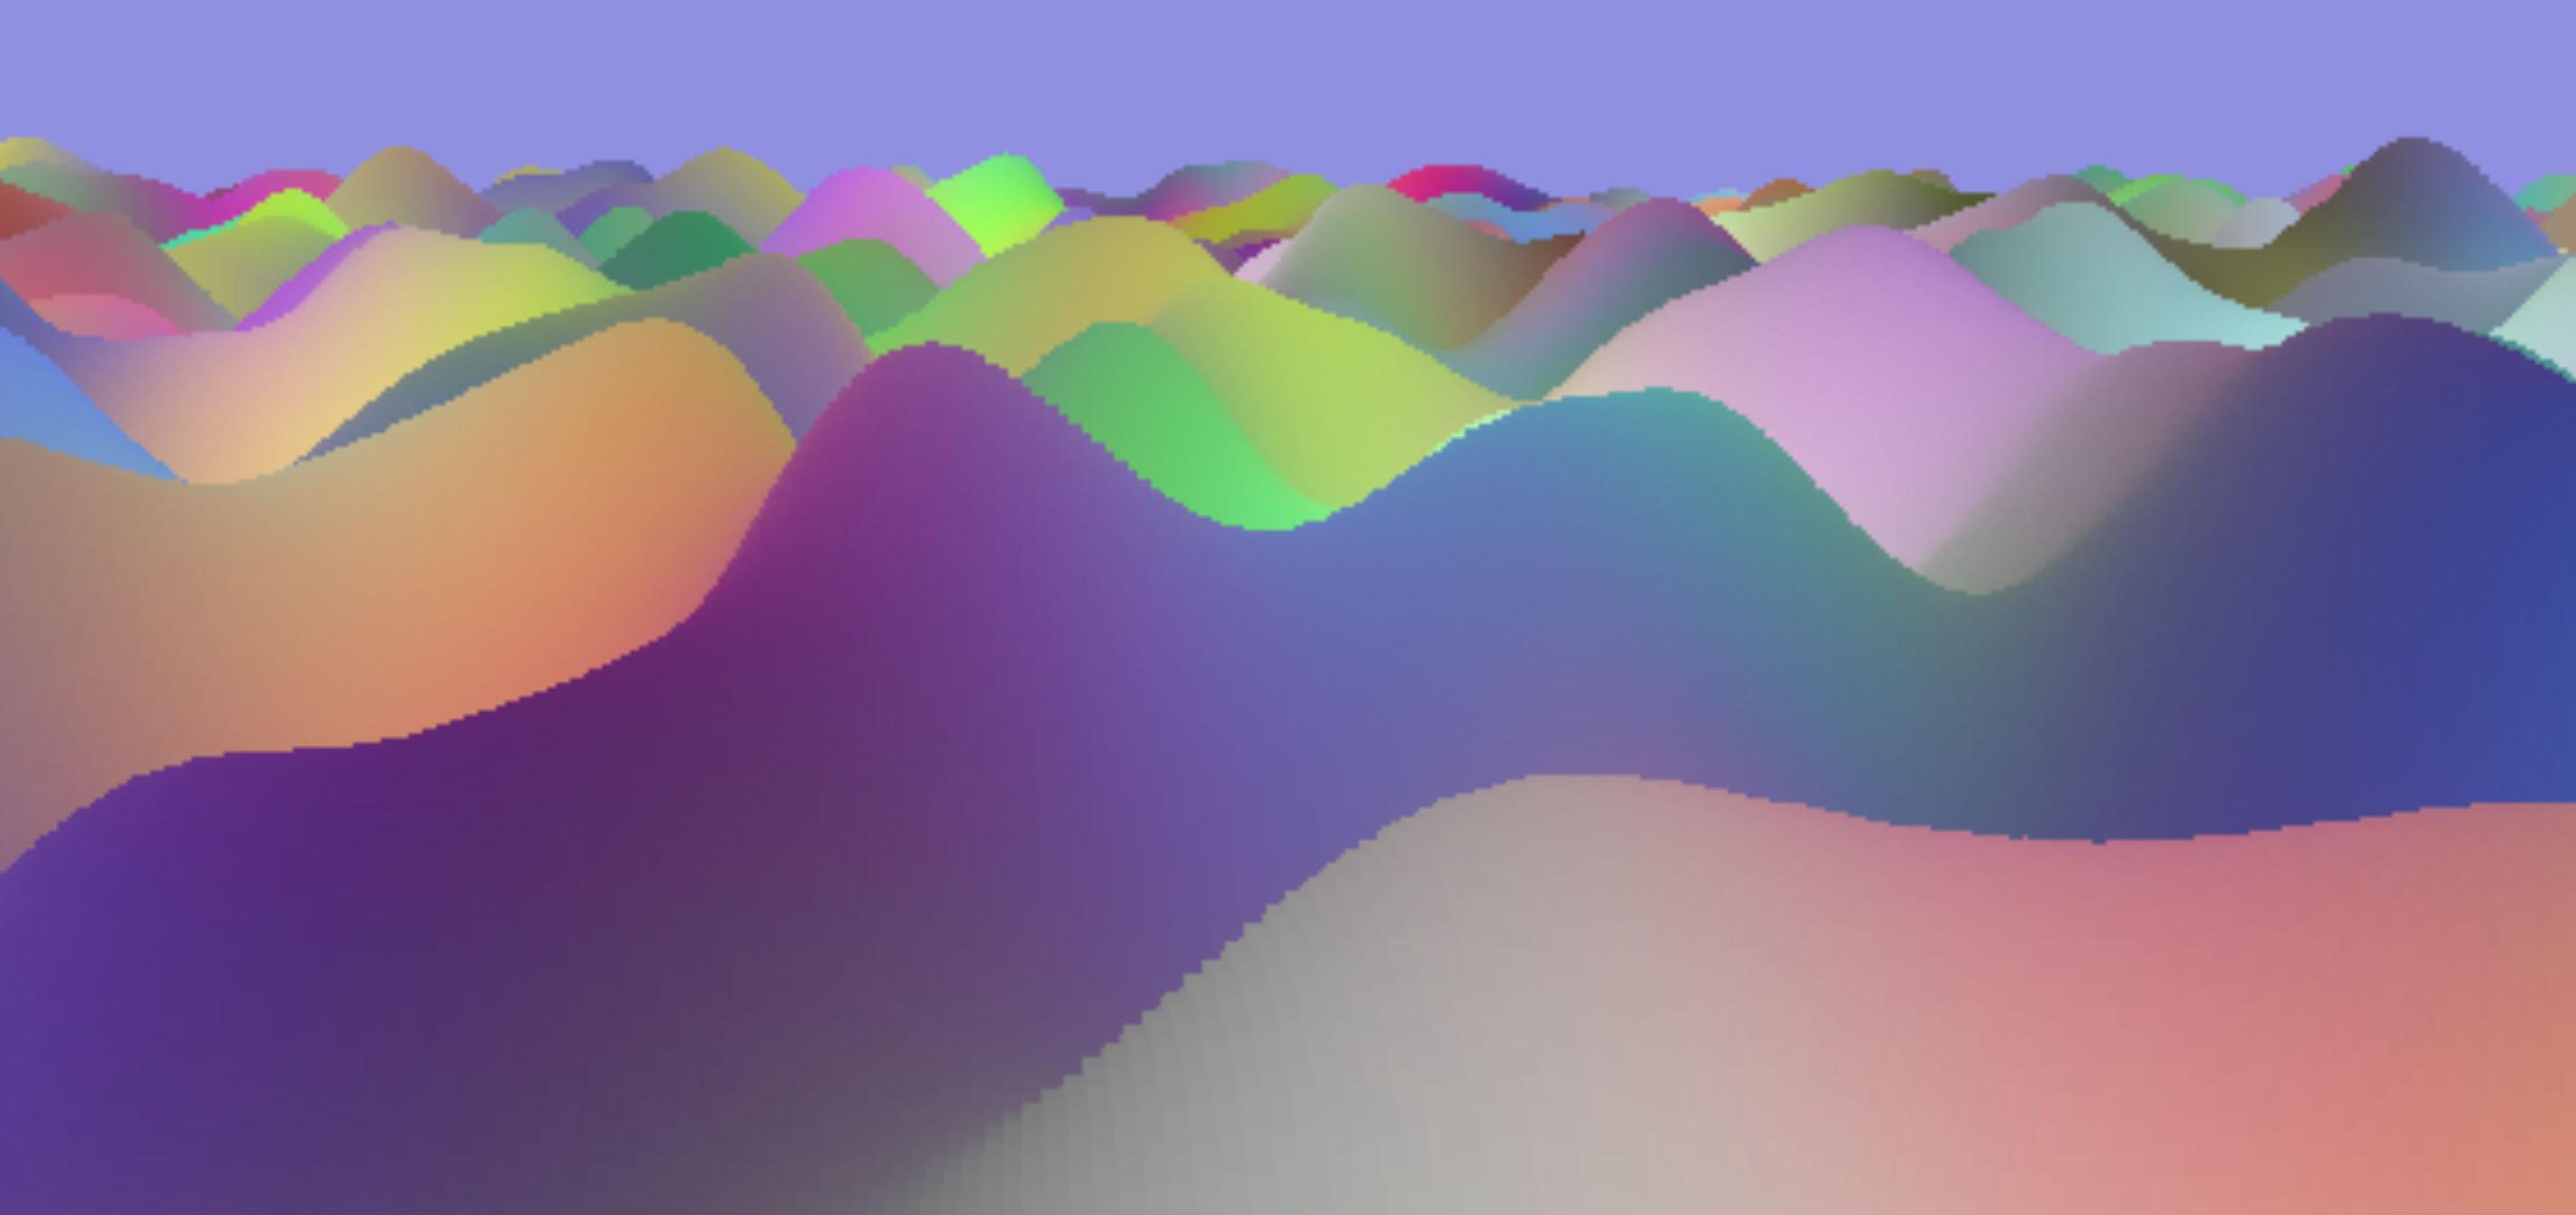
\includegraphics[scale=.15]{proc-voxel}
			\captionof{figure}{Rendering using the Voxel Space engine with a height and color map generated by Perlin noise.}
			\label{fig:pnvs}
		\end{minipage}
		
		The voxel space rendering engine originally utilized a pre-made height and color map to render from. This, combined with a tiling effect and knowledge of the field-of-view of the user's position allowed for a simplified three-dimensional rendering system. Starting from the furthest position to guarantee occlusion, a line on the map is determined in the triangular field of view. This is scaled with perspective projection, and a vertical line is drawn at every point on the screen from the section of the color map. The height of the vertical line is determined from the height drawn from the two-dimensional height map. Then, this is repeated until the entire field-of-view is drawn. This technique can be seen in \autoref{fig:vs-raster}. 
		
		\begin{minipage}{\textwidth}
			\centering
			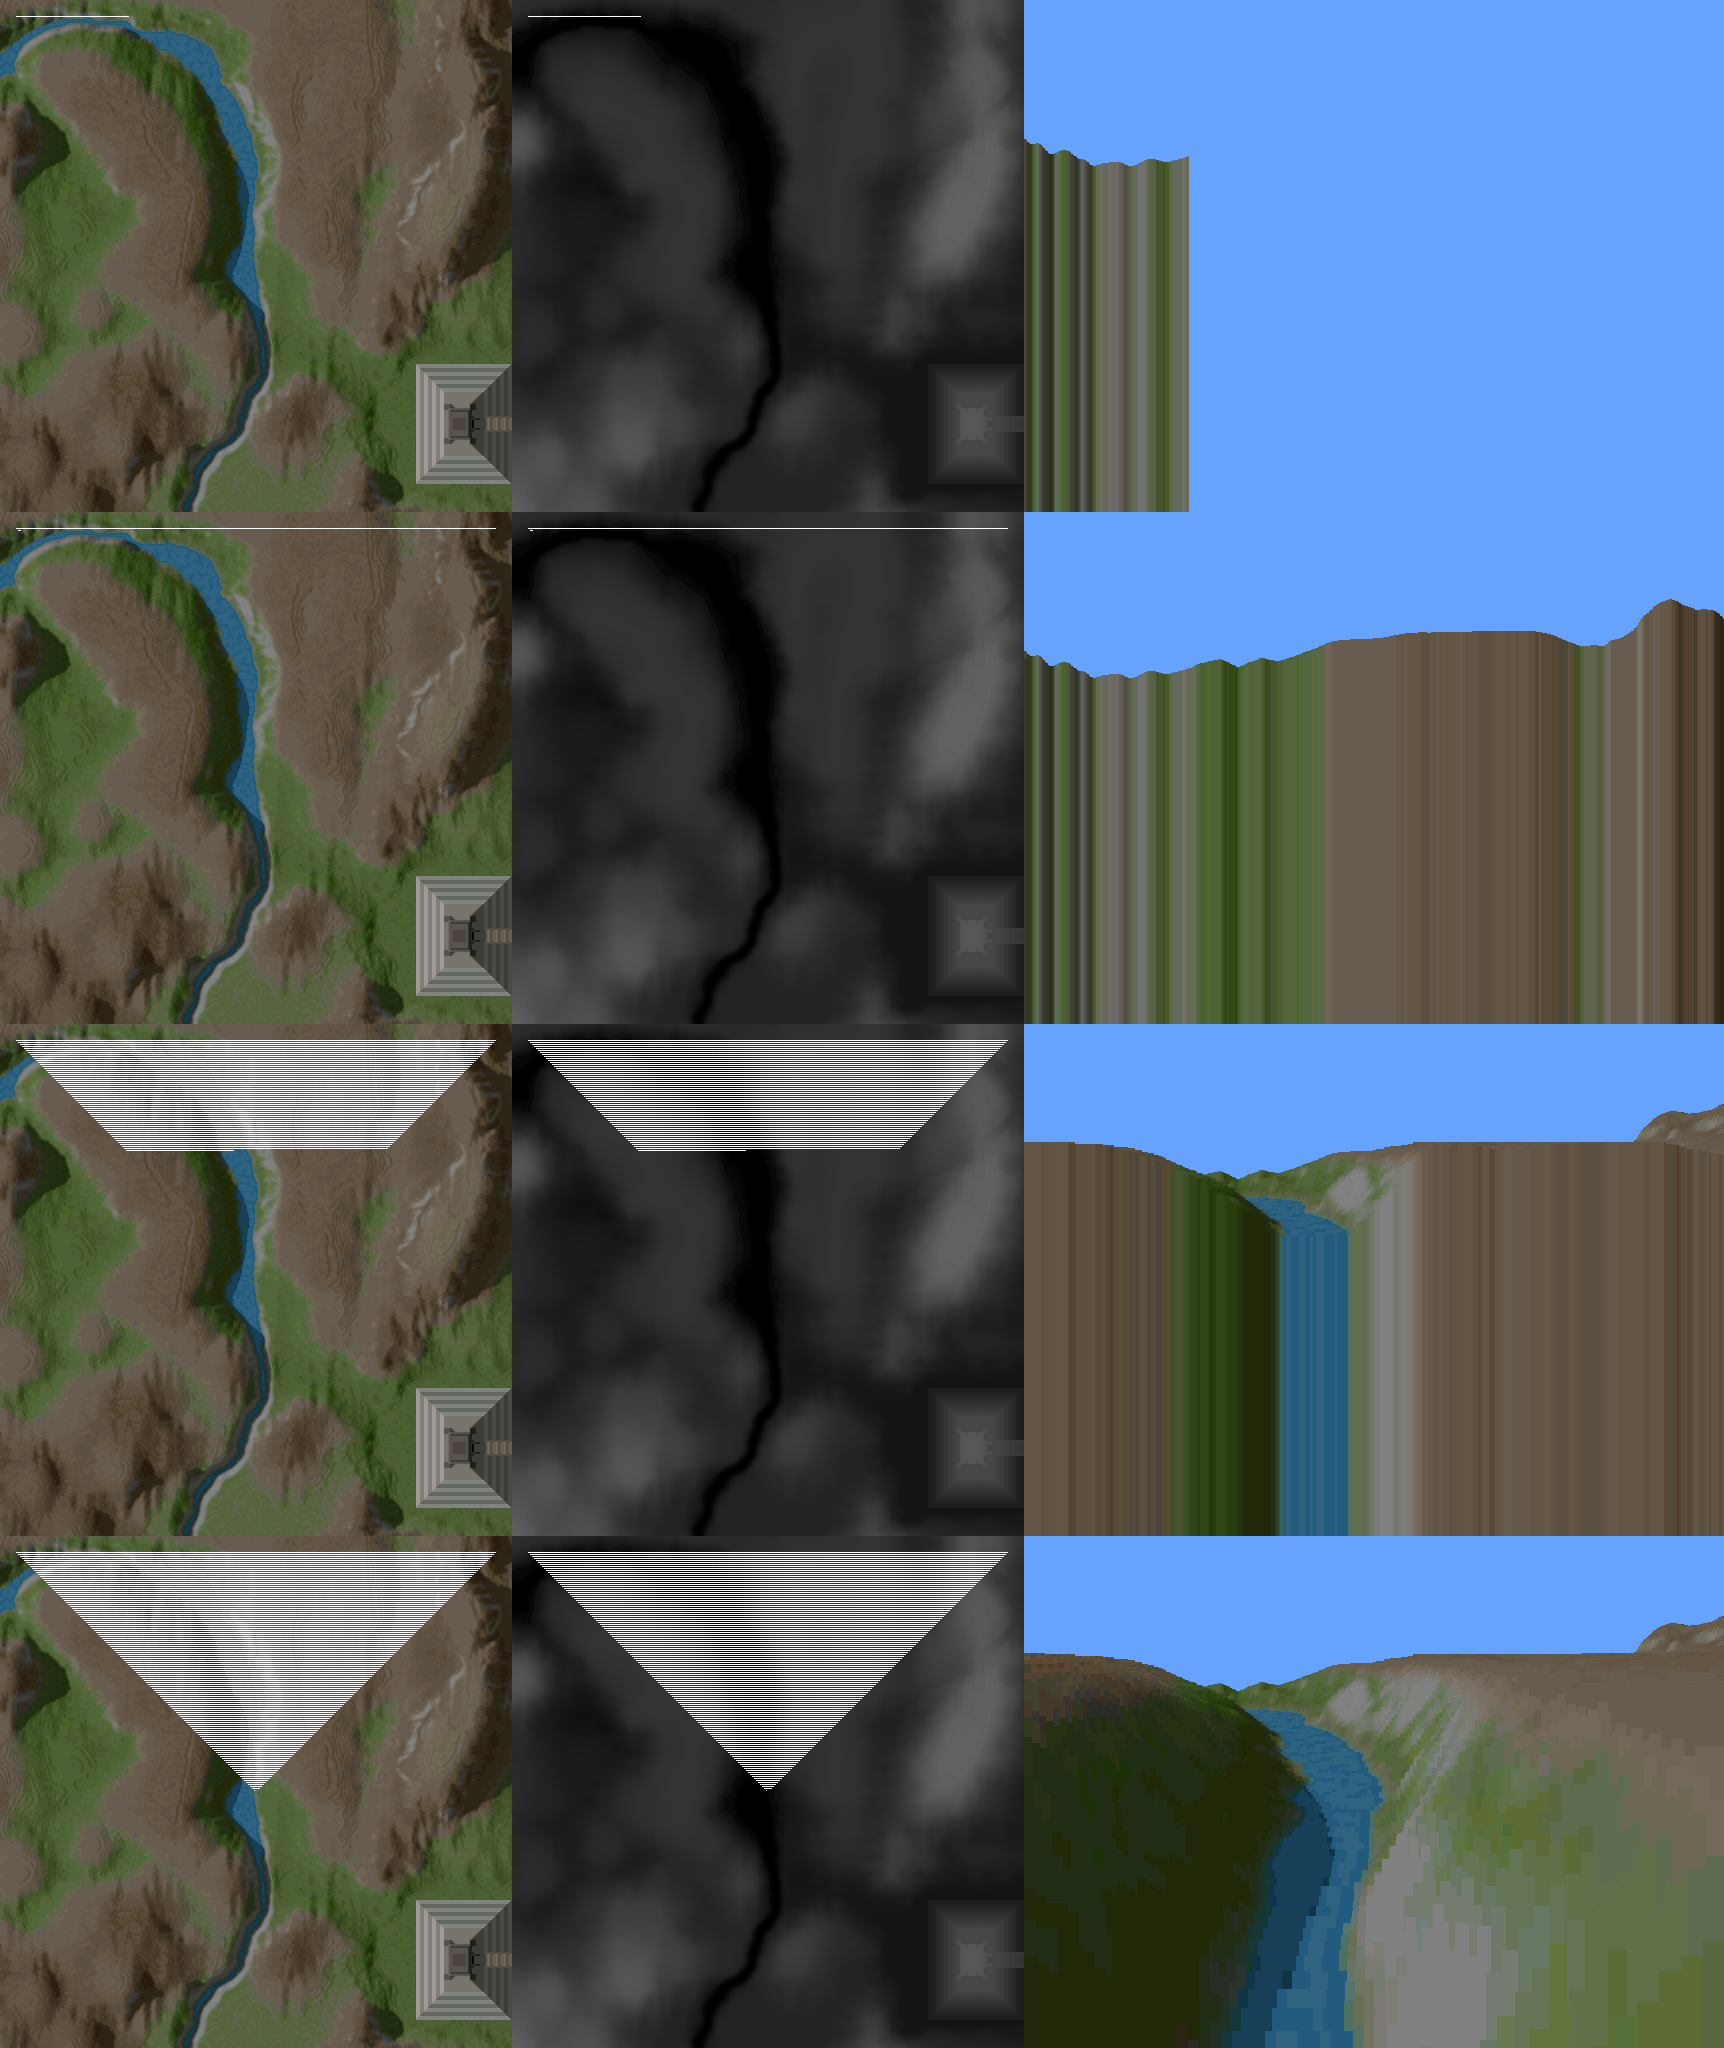
\includegraphics[scale=.2]{line-by-line}
			\captionof{figure}{Basic rasterization technique of the Voxel Space engine. \cite{voxel-space}}
			\label{fig:vs-raster}
		\end{minipage}
	
		This can be optimized with drawing from front-to-back with the addition of a y-buffer to determine the highest y position to draw. However, the voxel-space rendering system has a downside of having fewer pixels to determine the colors and heights of closer landmasses. This creates a pixellated effect for the foreground, while the background is rendered in higher detail. This method can be seen in more detail in \autoref{fig:vs-patent}. 
		 
		\begin{minipage}{\textwidth}
		 	\centering
		 	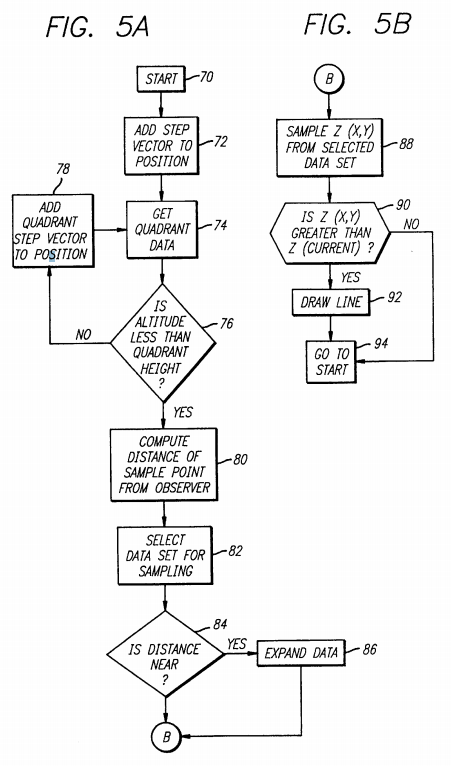
\includegraphics[scale=0.5]{US6020893A}
		 	\captionof{figure}{US Patent 6 020 893 \cite{US6020893}}
		 	\label{fig:vs-patent}
		\end{minipage}
		
		This weakness can be mitigated in some effect by having multiple heightmaps of differing detail to draw from. This would mitigate some of the advantage of voxel space rendering in increasing the rendering time and processing required for the algorithm. In addition to the weakness in rendering closer objects, height maps are also unable to render more complex geological formations, such as caves, archways or overhangs. Later iterations of the voxel space rendering engine worked around some of these limitations by introducing rendering of both polygons and voxels. Another possible workaround to the low resolution of the voxel space rendering system would be using procedurally generated noise as the platform for creating height maps. By creating the height map dynamically from noise, the memory used for storing the program overall would be smaller, and the resolution would not be constrained, as for areas closer to the camera, the interpolation between the points of the noise map would just be decreased. 	

	\vspace{10pt}
	\let\clearpage\relax	
	\chapter{Polygons}
	
		Polygons can be used as an alternative to image-based methods of rendering, or techniques like the voxel space engine. A polygon mesh is composed of three parts.
		
		\begin{center}
			\begin{tabular}{ l l } 
				V & a set of vertices (points in space)\\ 
				$E {\subset} (V x V)$ & a set of edges (line segments)\\ 
				$F {\subset} E*$  & a set of faces \\
			\end{tabular}
		\end{center}
		% https://www.classes.cs.uchicago.edu/archive/2015/fall/23700-1/docs/mesh-notes.pdf
	
		Now, with the increased processing power of computers and the optimizations made towards rendering these polygons, a polygon mesh will have thousands of individual vertices/triangles. Using these triangles, the computer is able to approximate a three-dimensional surface. For visibility, these polgyons can then be displayed with a front face and a back face, to calculate lighting and reduce some processing time. However, polygons have a similar rendering issue as height maps and image based methods. Since the polygons must be stored with a physical location, this means that every surface is typically just a sheet of paper. In rendering terrain, while polygons can render three dimensional terrain with overhangs and caves, these systems are almost always static. 
	
		\section{Rendering Differences}
		Polygons have a few notable disadvantages in the rendering of terrain. For example, given a two-dimensional array map or a noise height map, polygons can be used to connect each one of the points given in these maps to render all of the land faces. However, this causes some level of uniformity in the rendering system, as between each elevation grid, it is not possible to connect polygons in a way to create a truly vertical or horizonal slope. 
		
	
	\vspace{10pt}
	\let\clearpage\relax
	\chapter{Voxels}
	
		In contrast to polygons, voxels represent individual points in space. These indivudual points in space contain a few attributes, the position in space and typically the material and/or texture data among other things. This allows for easier computation of the absense of terrain data, such as in caves or polygons. In terms of creating a cave, the points in space representing the cave just need to be removed, in contrast to the mapping required to store the vertices in space. 
		
		\section{Rendering Differences}
		While voxels have advantages versus the use of polygons, they also have a number of disadvantages. Voxels require more memory to utilize properly. One example given is of a noise height map for a land that is 100m x 100m in size, with an elevation range from 0 to 100m. This information is stored using 32bit floats, requiring 320,000 bits of data, giving 100,000 points to connect using polygons. However, in contrast for the same noise height map, for each square meter of landscape on the screen of a 100x100 pixel monitor, the cubic meter would consist of 1,000,000 points for a memory requirement of 32,000,000,000,000 bits of data, over 100 million times the memory requirements of the polygon noise map. To alleviate this problem, voxel maps use a much larger polygonal cube size to reduce the memory requirements of using voxels \cite{high-level-voxel}. This leads into the use of voxels, and their blocky appearance in games such as Minecraft and Cubeworld.
		
		In addition, voxel-based rendering is not restricted to the use of noise or array maps to draw data from. Terrain can be definited by using a scalar function over a three-dimensional grid, also known as a voxel map. In a voxel map, the function value represents a form of distance from the terrain surface rather than elevation. For points in space outside of the terrain surface in empty space, the value would be positive, negative values would indicate that the point inside solid space, and a value of zero would correspond to the terrain's surface. This allows for greater topographical and topological complexity in representing the terrain. This improvement introduces its own difficulties, such as increasing the number of vertices and triangles needed to construct the terrain, increasing the development of a seamless algorithm for rendering the voxel based terrain, as well as increasing the texturing and shading from the possible complexity of the terrain. 
		
		\section{Blocky Voxels}
		While the success of Minecraft has made it the atypical example of procedural generation rendered using voxels, the representation of voxels as cubes stacked in space is not accurate to the greater definition of the voxels being points in space. Minecraft does use a voxel system to store the points in space as data, indexed by an YZX system for compression \cite{minecraft-voxel}. However, Minecraft's rendering system is based around a polygon system to display the individual blocks. 
		
		\section{Examples}
		
	
	\vspace{10pt}
	\let\clearpage\relax
	\chapter{Development}

		\section{Areas of Research}
	
		An ongoing area of research for PGC is the introduction of neural networks as the framework, instead of more traditional algorithms or techniques. One example of this is the procedural generation of terrain via Tensorflow. This impementation was trained on a large dataset of terrain height maps, around 10,000, with the addition of satellite data to use for coloring. The specific neural network involved in the implementation was a Generative Adversarial network, which works on creating fake images, and attempting to discern between real and fake. By iterating this, the network will get better at both tasks, with the generator learning how to create more and more realistic images. For the problem of coloring the terrain, a style network was used to take two images and blend them to create an output image that looks like the content image, but with the style of the reference image. This technique is used in other applications, such as the neural networks trained on recreating photographs in a particular artist's style, shown in \autoref{fig:neural-style}. 
		
		\begin{minipage}{\textwidth}
			\centering
			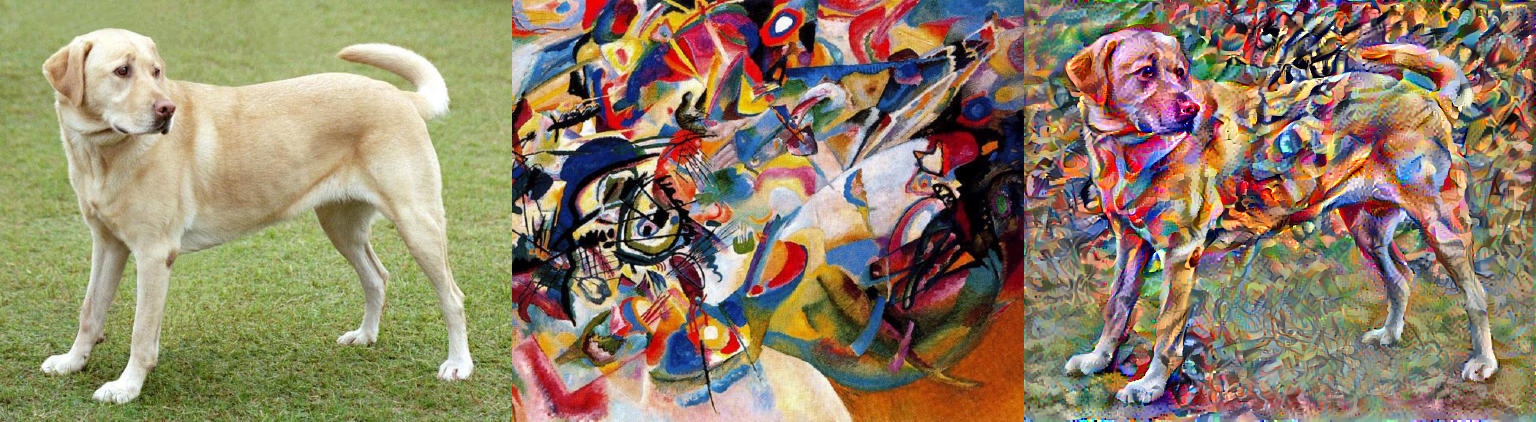
\includegraphics[scale=.3]{stylized-image}
			\captionof{figure}{An example of neural style transfer \cite{tf-style}}
			\label{fig:neural-style}
		\end{minipage}
	
		The initial processing pipeline utilized convolutional transpose to generate the output height and colormaps. However, this approach led to grid-like artifacting due to the misaligned output size compared to the kernel size. The solution used for combatting this was bilinear sampling, by adding pixels from surrounding pixels to determine value rather than the kernels and strides. While the resultant height maps are impressive, additional research is likely required to determine differences between this approach and another approach such as Simplex noise. In \autoref{fig:dl-noise}, the results can be seen. 
		
		\begin{minipage}{\textwidth}
			\centering
			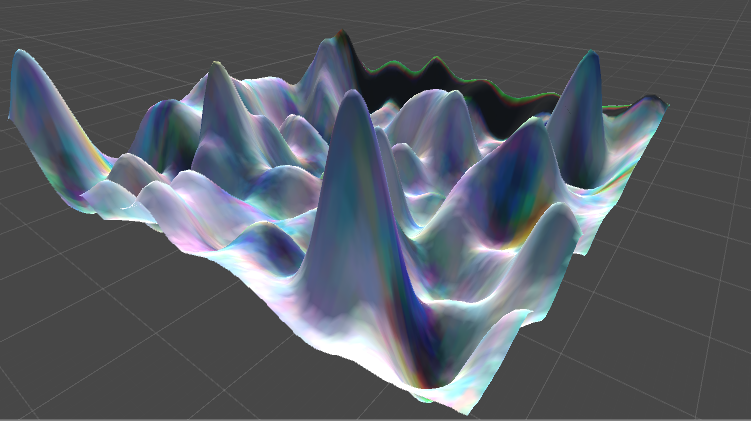
\includegraphics[scale=.3]{rolling}
			\captionof{figure}{Example of three-dimensional worlds created with deep learning \cite{nn-noise}}
			\label{fig:dl-noise}
		\end{minipage}
	
		The field of procedural content generation using machine learning is constantly evolving, as there are many different methodologies that have been applied to this task. The multitude of neural architectures allows for the tailoring of neural networks to different types of generated content, at the cost of necessitating large amounts of searching for the right architectures.
		
		\cite{Liu_2020}
		
		\section{Algorithm Advancements}
		
		Perlin noise was designed to address some of the limitations of the original Perlin noise. Since the original implementation of Perlin noise was constrained by the lattice gradient function creating directional artifacts, one of the goals of Simplex noise was to overcome this limitation. In addition, Simplex noise has lower computational complexity - O(k\textsuperscript{2}) instead of O(2\textsuperscript{k})\cite{sheet-simplex}. Other benefits includes the capability to scale to higher dimensions, a well-defined and continuous gradient, as well as simpler implementation. Instead of the lattice gradients that Perlin noise works on, Simplex noise works based on simplex grids for which it was named after. This involves choosing the simplest, repeatable shape to fill a N-dimensional space. Another definition of a n-simplex would be it being the smallest figure that contains n+1 given points in n-dimensional space, while not lying in the space of a lower dimension. In one dimension, this works by choosing repeating line segments. In two dimensions, this becomes an equilateral triangle. In three dimensions, this becomes a trianglular pyramid, also known as a tetrahedron. From four dimensions and onward, this simplex becomes increasingly difficult to visualize. However, there is a pattern in the drawability of simplexes, by creating a new point and connecting it to all previously existing points.
		
		\begin{minipage}{\textwidth}
			\centering
			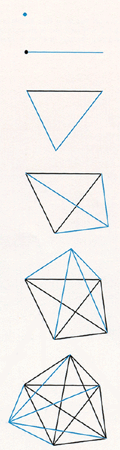
\includegraphics[scale=.75]{six simplexes}
			\captionof{figure}{The first six simplexes \cite{higher-dim-simplexes}}
			\label{fig:fig2}
		\end{minipage}
	
		The relative simplicity of the simplex shape in having as few corners as possible makes it a lot easier to interpolate values in the interior of the shape, relative to the hypercubes used in the original Perlin noise.
		In the original Perlin noise function, derivatives were used to compute the gradation between the points. This creates a large increase in computational complexity based on dimensionality. Simplex noise instead uses the summation of kernel values to determine the point's value. To generate the Simplex noise, the value for any point in space must be determined. In two dimensional space, this means skewing the coordinate space along the main diagonal, transforming the squashed equilateral triangles into right-angle isosceles triangles. From there, determining the location is made more simple, as just the integer part of the coordinates is needed for each dimension. Beyond two dimensions, the visualization becomes more difficult, but the methods remain the same.  
		
		\begin{minipage}{\textwidth}
			\centering
			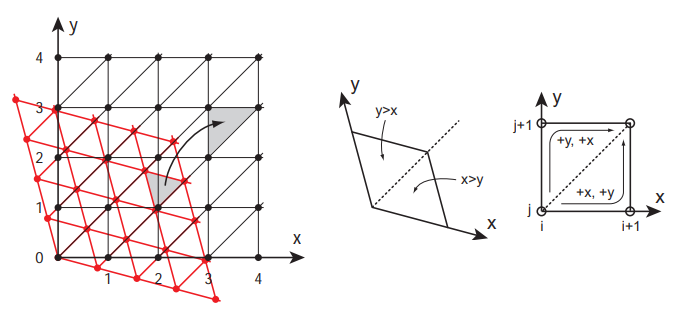
\includegraphics[scale=.5]{skewed grid}
			\captionof{figure}{Skewing in two-dimensional space and determining the cell containing a point. \cite{simplex-demyst}}
			\label{fig:fig9}
		\end{minipage}
		
		The traversal scheme for a two-dimensional simplex is built around this triangular method. If the x and y coordinates are known, then all that is needed is to determine which of the two simplices the point lies in. If x > y, the corners become (0,0), (1,0) and (1,1), else the corners are (0,0), (0,1) and (1,1). To traverse this, only one step in the x and one step in the y is needed, but in a different order for each of the simplices. This technique can then be generalized to any arbitrary amount of N dimensions \cite{simplex-demyst}. While Perlin noise has many advantages over the classical Perlin noise, it has a different visual characteristic, making it difficult to directly replace or compare the two. 
		
		\begin{minipage}{\textwidth}
			\centering
			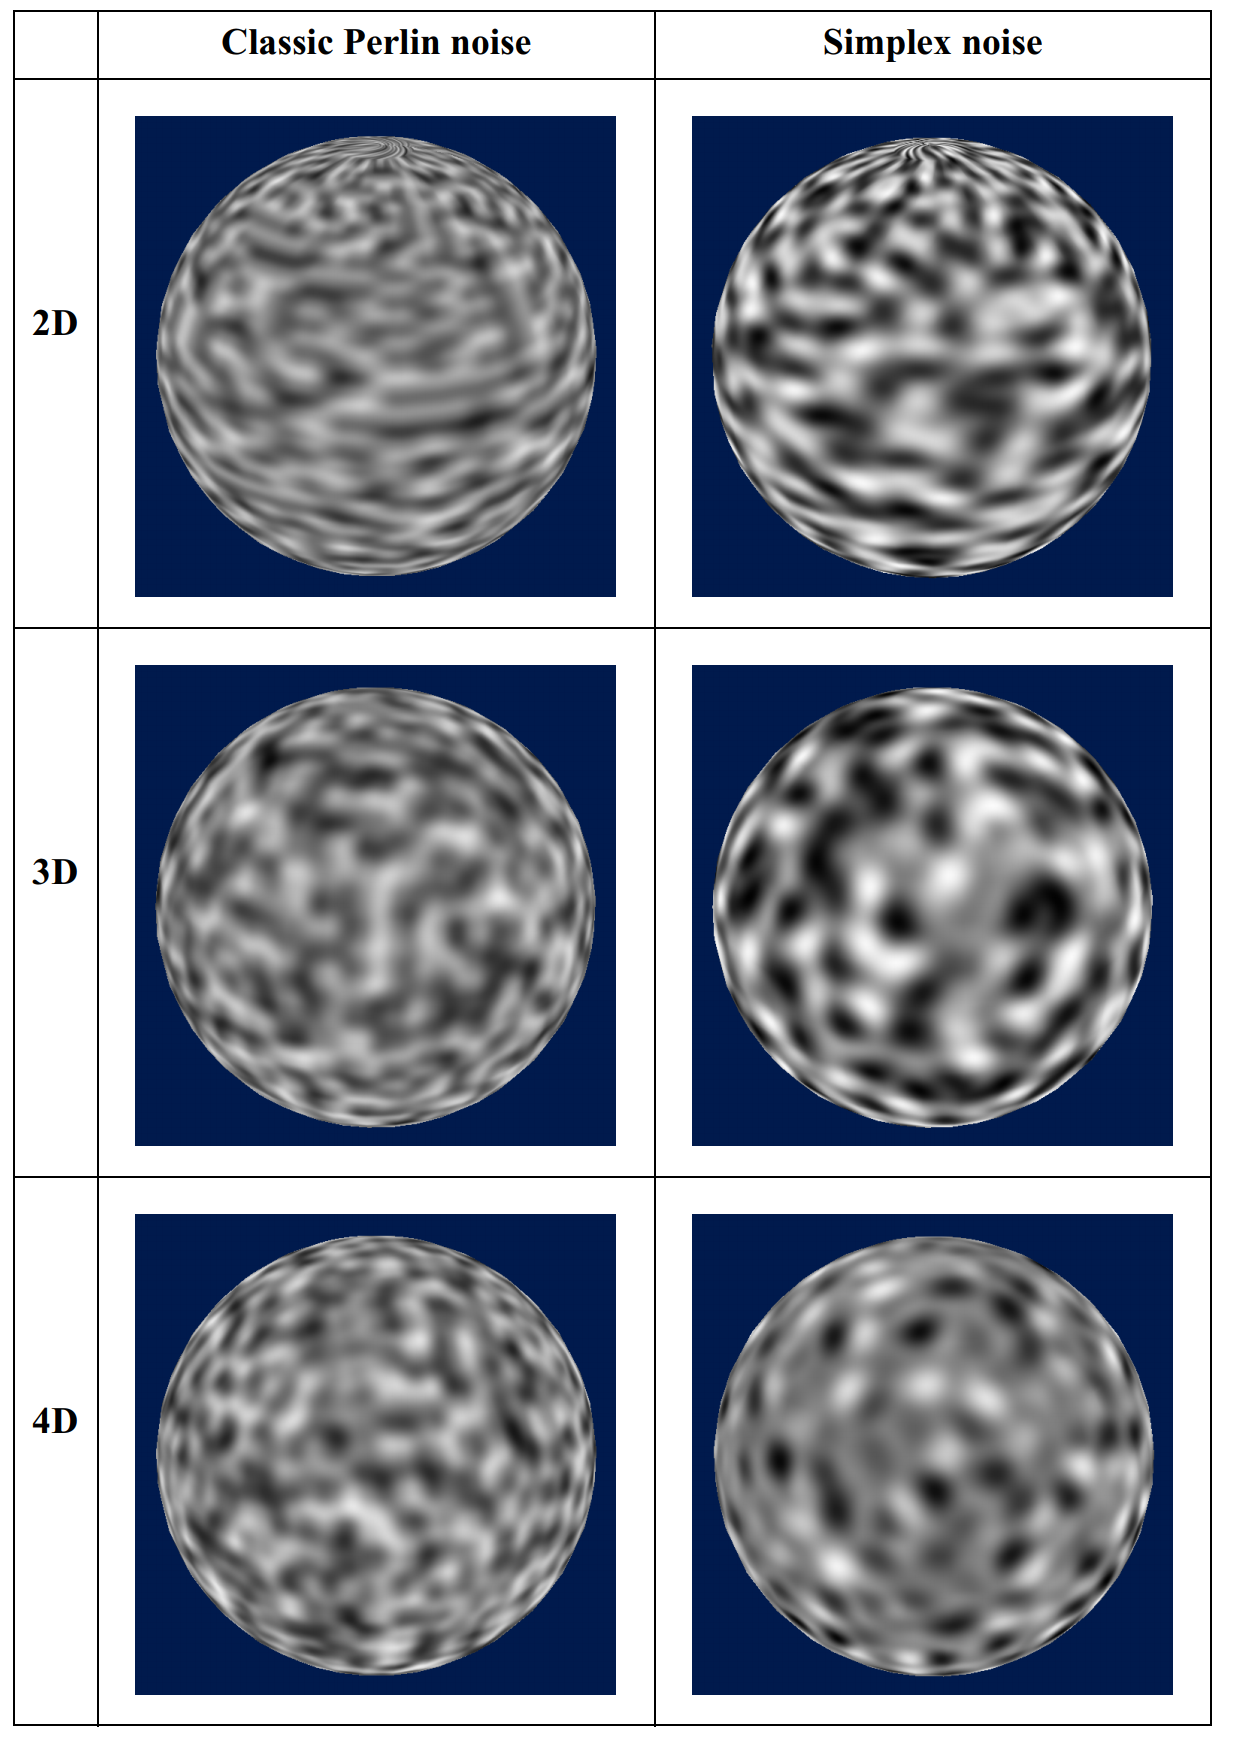
\includegraphics[scale=.25]{perlin vs simplex}
			\captionof{figure}{A comparison of Perlin and Simplex noise \cite{simplex-demyst}}
			\label{fig:fig4}
		\end{minipage}
	
		However, with additional modification using multiple layers or octaves, Simplex noise will run much more computationally efficiently, as well as replicating the visual quirks of Perlin noise. 
		
		In addition to the advancements in noise generation, rendering techniques associated with procedural generation have had advancements as well. For example voxel-based terrain has had advances in both the front and back-end of the algorithms. Voxel-based rendering methods often use a marching cubes algorithm to both smooth voxel surfaces and increase runtimes. A modified version of this algorithm was created to facilitate faster implementation and design of a level-of-detail algorithm. Some of the difficulties of this revised implementation of the Marching Cubes algorithm involved finding a suitable compression technique for the voxel map, as for larger terrains, voxel mapping will quickly grow beyond the limits of addressable memory. In addition, limiting the density of vertices, triangles and individual meshes through a level-of-detail system ensures the higher rendering performance of this revised algorithm. 
		
		The modified Marching Cubes combined with a Transition Cubes algorithm provides a method for stitching together voxel-based meshes and eliminating seams.R endering the areas of a terrain at different detail layers allows for efficient usage of processing power, but introduces the problem of seams between the cells. This problem can be shown in \autoref{fig:voxel-artifact}. 
		
		\begin{minipage}{\textwidth}
			\centering
			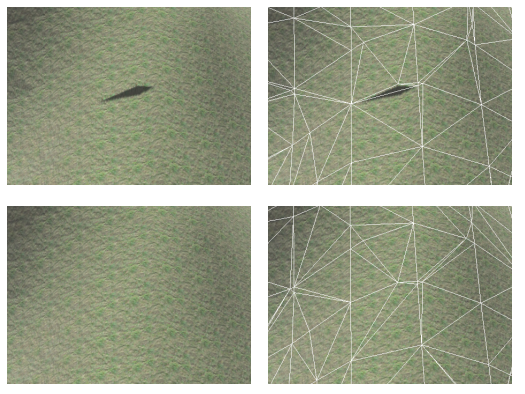
\includegraphics[scale=.75]{voxel-seam}
			\captionof{figure}{A shadow artifact fixed with transition cells \cite{10.5555/1925140}}
			\label{fig:voxel-artifact}
		\end{minipage}
		
		The Transition Cubes method developed in this paper utilizes transition cells inserted in between ordinary cells of a voxel map. This efficiently generates the triangles to connect terrain blocks rendered at different levels of detail, as modifications to one level of detail means that all levels must be adjusted to remain consistent, with the mapping of these different layers shown in \autoref{fig:voxel-layered-mapping}.
		
		\begin{minipage}{\textwidth}
			\centering
			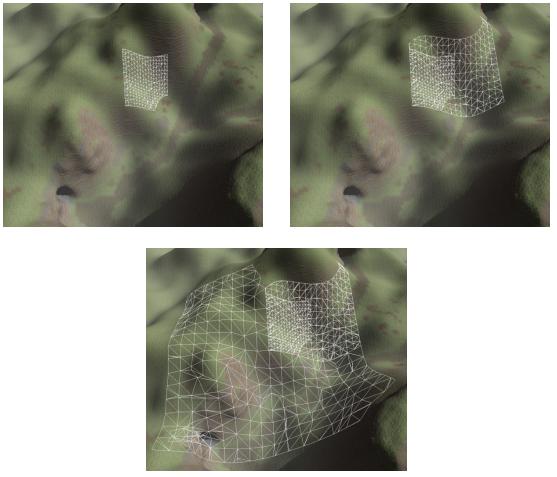
\includegraphics[scale=.75]{voxel-detail}
			\captionof{figure}{Layered resolution details of voxel meshes \cite{10.5555/1925140}}
			\label{fig:voxel-layered-mapping}
		\end{minipage}
		% URL holder http://transvoxel.org/Lengyel-VoxelTerrain.pdf
			
	\vspace{10pt}
	\let\clearpage\relax
	\chapter{Summary}
		
		While procedural generation has a background based in signals processing and mathematics, its usage has extended far beyond these fields in the creation of procedurally generated worlds, stories, characters and more. The procedural generation of geological formations in particular is a difficult problem, as rendering and storing the terrain data in memory proves to be a challenge for any approach of procedural generation. In recent years, the voxel approach has supplanted previous techniques and has become more widespread. However, the fundamental algorithms and processes to create noise have remained largely the same, with improvements. Some of these techniques include Perlin noise, Fractal Geometry and Cellular Automata. These techniques have been used to create different sorts of maps in attempts to create two and three-dimensional landscapes. To render the data created from these processes, image-based, polygonal and voxel techniques have been applied, with varying strengths and weaknesses. Image-based techniques have the advantage of low computational requirements and simplicity of implementation, but have the drawbacks of being reliant on either a pre-determined, procedurally generated image, or having an excess of pseudo-random algorithms always running in the background. In contrast, while polygons are a common method for rendering non procedurally generated games, it has several drawbacks with a randomly created space. Interpreting the data from this space becomes a challenge, as well as creating more three-dimensional structures, as polygons have difficulty in creating certain slopes and landscape geometries. Voxels alleviate the problems in geometric representation, but come with the downsides of excessive processing and memory usage, in addition to having issues with tiling. However, for all of these methods, several advancements have been made to mitigate or address these issues. 
	
	\newpage
	\renewcommand{\bibname}{References}
	\bibliographystyle{plain}
	\bibliography{refs} % Entries are in the "refs.bib" file
		
\end{document}